\section{ZLIM Adjust Z Axis limits of plot}

\subsection{Usage}

There are several ways to use \verb|zlim| to adjust the Z axis limits of
a plot.  The various syntaxes are
\begin{verbatim}
   zlim
   zlim([lo,hi])   
   zlim('auto')
   zlim('manual')
   zlim('mode')
   zlim(handle,...)
\end{verbatim}
The first form (without arguments), returns a 2-vector containing the
current limits.  The second form sets the limits on the plot to \verb|[lo,hi]|.
The third and fourth form set the mode for the limit to \verb|auto| and \verb|manual|
respectively.  In \verb|auto| mode, FreeMat chooses the range for the axis 
automatically.  The \verb|zlim('mode')| form returns the current mode for the axis
(either \verb|'auto'| or \verb|'manual'|).  Finally, you can specify the handle of an
axis to manipulate instead of using the current one.
\subsection{Example}

\begin{verbatim}
--> x = linspace(-1,1);
--> y = sin(2*pi*x);
--> plot(x,y,'r-');
--> zlim  % what are the current limits?

ans = 
   -0.5000    0.5000 
\end{verbatim}
which results in


\centerline{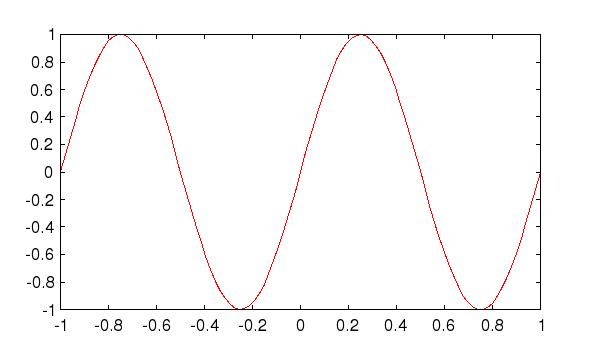
\includegraphics[width=8cm]{zlim1}}

Next, we zoom in on the plot using the \verb|zlim| function
\begin{verbatim}
--> plot(x,y,'r-')
--> zlim([-0.2,0.2])
\end{verbatim}
which results in


\centerline{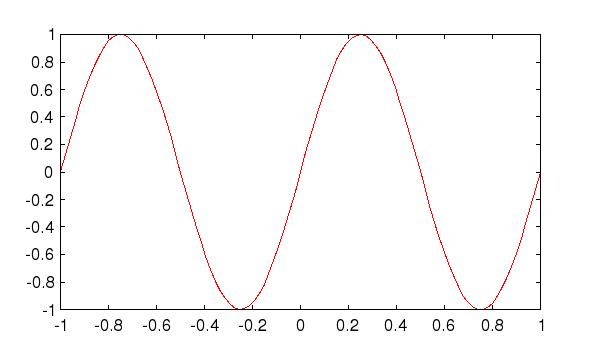
\includegraphics[width=8cm]{zlim2}}

